%%%%%%%%%%%%%%%%%%%%%%%%%%%%%%%%%
% baposter Landscape Poster
% LaTeX Template
% Version 1.0 (15/5/13)
%
% Created by:
% Brian Amberg (baposter@brian-amberg.de)
%
% This template has been downloaded from:
% http://www.LaTeXTemplates.com
%
% License:
% CC BY-NC-SA 3.0 (http://creativecommons.org/licenses/by-nc-sa/3.0/)
%
%%%%%%%%%%%%%%%%%%%%%%%%%%%%%%%%%%%%%%%%%

%----------------------------------------------------------------------------------------
%	PACKAGES AND OTHER DOCUMENT CONFIGURATIONS
%----------------------------------------------------------------------------------------

\documentclass[paperwidth=36in,paperheight=48in,portrait,fontscale=0.355, margin=2cm]{baposter}

\usepackage[utf8]{inputenc}
\usepackage[font=normalsize,labelfont=bf]{caption} % Required for specifying captions to tables and figures
\captionsetup{justification=centering}
\usepackage{booktabs} % Horizontal rules in tables
\usepackage{lmodern}
\usepackage{relsize} % Used for making text smaller in some places

% Other packages
\usepackage{tabularx}
\def\tabularxcolumn#1{m{#1}}
\def\imagetop#1{\vtop{\null\hbox{#1}}}
\usepackage{adjustbox}
\usepackage{subfig}
\usepackage{floatrow} % sidecapfloat
\usepackage{setspace}
\usepackage{xspace}
\usepackage{noReferences}
\usepackage{caption}
\usepackage{tikz}
\usepackage[customcolors]{hf-tikz}
%\usepackage{subcaption}
\usepackage{epsf}
\usepackage{amsmath}
\usepackage{mathtools}
\usepackage{amssymb}
\usepackage{amsfonts}
\usepackage{amsthm}
\usepackage{dsfont}
\usepackage{enumitem}
\usepackage{float}
\usepackage{cases}
\usepackage{verbatim}
\usepackage{array}
\usepackage{graphicx}
\usepackage{graphics}
\usepackage{multirow}
\usepackage{listings}
%\usepackage[authoryear]{natbib}
\usepackage{authblk}
\usepackage[linesnumbered,ruled,vlined]{algorithm2e}
\usepackage{eqparbox}
\usepackage{xcolor}
\usepackage[backend=biber, citestyle=authoryear, maxcitenames=2, maxbibnames=2]{biblatex}
\usepackage{lipsum}
\usepackage{svg}
\usepackage{cleveref}
\usepackage{pifont} 

\renewcommand\thefootnote{\alph{footnote}}

\bibliography{../references.bib}

\definecolor{darkspringgreen}{rgb}{0.09, 0.45, 0.27}
\definecolor{cadmiumgreen}{rgb}{0.0, 0.42, 0.24}
\newcommand{\hlr}[1]{\textcolor{Red}{#1}}
\newcommand{\hlb}[1]{\textcolor{Blue}{#1}}
\newcommand{\hlg}[1]{\textcolor{cadmiumgreen}{#1}}
\newcommand{\hlm}[1]{\textcolor{BurntOrange}{#1}}


%%%%%%%%%%%%%%%%%%%%%%%%%%%%
% Paper dependent stuff    %
%%%%%%%%%%%%%%%%%%%%%%%%%%%%

\newcommand{\Tau}{\mathcal{T}}

%%%%%%%%%%%%%%%%%%%%%%%%%%%%
% Aesthetics               %
% over-underline, hat, bold%
%%%%%%%%%%%%%%%%%%%%%%%%%%%%

\newcommand{\eps}{\varepsilon}
\newcommand{\vareps}{\varepsilon}
\renewcommand{\epsilon}{\varepsilon}
%\renewcommand{\hat}{\widehat}
\renewcommand{\tilde}{\widetilde}
\renewcommand{\bar}{\overline}

\newcommand*{\MyDef}{\mathrm{\tiny def}}
\newcommand*{\eqdefU}{\ensuremath{\mathop{\overset{\MyDef}{=}}}}% Unscaled version
% \newcommand*{\eqdef}{\mathop{\overset{\MyDef}{\resizebox{\widthof{\eqdefU}}{\heightof{=}}{=}}}}
\newcommand{\eqdef}{\stackrel{def}{=}}


\def\:#1{\protect \ifmmode {\mathbf{#1}} \else {\textbf{#1}} \fi}
\newcommand{\CommaBin}{\mathbin{\raisebox{0.5ex}{,}}}

\newcommand{\wt}[1]{\widetilde{#1}}
\newcommand{\wh}[1]{\widehat{#1}}
\newcommand{\wo}[1]{\overline{#1}}
\newcommand{\wb}[1]{\overline{#1}}

% bf and bm missing due to conflict!!
\newcommand{\bsym}[1]{\mathbf{#1}}
\newcommand{\bzero}{\mathbf{0}}
\newcommand{\ba}{\mathbf{a}}
\newcommand{\bb}{\mathbf{b}}
\newcommand{\bc}{\mathbf{c}}
\newcommand{\bd}{\mathbf{d}}
\newcommand{\be}{\mathbf{e}}
\newcommand{\bg}{\mathbf{g}}
\newcommand{\bh}{\mathbf{h}}
\newcommand{\bi}{\mathbf{i}}
\newcommand{\bj}{\mathbf{j}}
\newcommand{\bk}{\mathbf{k}}
\newcommand{\bl}{\mathbf{l}}
\newcommand{\bn}{\mathbf{n}}
\newcommand{\bo}{\mathbf{o}}
\newcommand{\bp}{\mathbf{p}}
\newcommand{\bq}{\mathbf{q}}
\newcommand{\br}{\mathbf{r}}
\newcommand{\bs}{\mathbf{s}}
\newcommand{\bt}{\mathbf{t}}
\newcommand{\bu}{\mathbf{u}}
\newcommand{\bv}{\mathbf{v}}
\newcommand{\bw}{\mathbf{w}}
\newcommand{\bx}{\mathbf{x}}
\newcommand{\by}{\mathbf{y}}
\newcommand{\bz}{\mathbf{z}}

\newcommand{\bA}{\mathbf{A}}
\newcommand{\bB}{\mathbf{B}}
\newcommand{\bC}{\mathbf{C}}
\newcommand{\bD}{\mathbf{D}}
\newcommand{\bE}{\mathbf{E}}
\newcommand{\bF}{\mathbf{F}}
\newcommand{\bG}{\mathbf{G}}
\newcommand{\bH}{\mathbf{H}}
\newcommand{\bI}{\mathbf{I}}
\newcommand{\bJ}{\mathbf{J}}
\newcommand{\bK}{\mathbf{K}}
\newcommand{\bL}{\mathbf{L}}
\newcommand{\bM}{\mathbf{M}}
\newcommand{\bN}{\mathbf{N}}
\newcommand{\bO}{\mathbf{O}}
\newcommand{\bP}{\mathbf{P}}
\newcommand{\bQ}{\mathbf{Q}}
\newcommand{\bR}{\mathbf{R}}
\newcommand{\bS}{\mathbf{S}}
\newcommand{\bT}{\mathbf{T}}
\newcommand{\bU}{\mathbf{U}}
\newcommand{\bV}{\mathbf{V}}
\newcommand{\bW}{\mathbf{W}}
\newcommand{\bX}{\mathbf{X}}
\newcommand{\bY}{\mathbf{Y}}
\newcommand{\bZ}{\mathbf{Z}}

% calligraphic
\newcommand{\cf}{\mathcal{f}}
\newcommand{\cA}{\mathcal{A}}
\newcommand{\cB}{\mathcal{B}}
\newcommand{\cC}{\mathcal{C}}
\newcommand{\cD}{\mathcal{D}}
\newcommand{\cE}{\mathcal{E}}
\newcommand{\cF}{\mathcal{F}}
\newcommand{\cG}{\mathcal{G}}
\newcommand{\cH}{\mathcal{H}}
\newcommand{\cI}{\mathcal{I}}
\newcommand{\cJ}{\mathcal{J}}
\newcommand{\cK}{\mathcal{K}}
\newcommand{\cL}{\mathcal{L}}
\newcommand{\cM}{\mathcal{M}}
\newcommand{\cN}{\mathcal{N}}
\newcommand{\cO}{\mathcal{O}}
\newcommand{\cP}{\mathcal{P}}
\newcommand{\cQ}{\mathcal{Q}}
\newcommand{\cR}{\mathcal{R}}
\newcommand{\cS}{\mathcal{S}}
\newcommand{\cT}{\mathcal{T}}
\newcommand{\cU}{\mathcal{U}}
\newcommand{\cV}{\mathcal{V}}
\newcommand{\cW}{\mathcal{W}}
\newcommand{\cX}{\mathcal{X}}
\newcommand{\cY}{\mathcal{Y}}
\newcommand{\cZ}{\mathcal{Z}}

%%%%%%%%%%%%%%%%%%%%%%%%%%%%
% Math jargon              %
%%%%%%%%%%%%%%%%%%%%%%%%%%%%
\newcommand{\wrt}{w.r.t.\xspace}
\newcommand{\defeq}{\stackrel{\mathclap{\normalfont\mbox{\tiny def}}}{=}}
\newcommand{\maxund}[1]{\max\limits_{#1}}
\newcommand{\supund}[1]{\text{sup}\limits_{#1}}
\newcommand{\minund}[1]{\min\limits_{#1}}
\renewcommand{\epsilon}{\varepsilon}
\newcommand{\bigotime}{\mathcal{O}}


\DeclareMathOperator*{\argmin}{arg\,min} 
\DeclareMathOperator*{\argmax}{arg\,max} 
\DeclareMathOperator*{\cupdot}{\mathbin{\mathaccent\cdot\cup}}

%%%%%%%%%%%%%%%%%%%%%%%%%%%%
% Matrix operators         %
%%%%%%%%%%%%%%%%%%%%%%%%%%%%
\newcommand{\transpose}{^\mathsf{\scriptscriptstyle T}}
\newcommand{\transp}{\mathsf{\scriptscriptstyle T}}
\DeclareMathOperator{\Tr}{Tr}
\DeclarePairedDelimiterX{\inp}[2]{\langle}{\rangle}{#1, #2}

%%%%%%%%%%%%%%%%%%%%%%%%%%%%
% Statistic operators      %
%%%%%%%%%%%%%%%%%%%%%%%%%%%%
\newcommand{\probability}[1]{\mathbb{P}\left(#1\right)}
\newcommand{\probdist}{Pr}
\DeclareMathOperator*{\expectedvalue}{\mathbb{E}}
\DeclareMathOperator*{\variance}{\text{Var}}
\newcommand{\expectedvalueover}[1]{\expectedvalue\limits_{#1}}
\newcommand{\condbar}{\;\middle|\;}
\newcommand{\gaussdistr}{\mathcal{N}}
\newcommand{\uniformdistr}{\mathcal{U}}
\newcommand{\bernoullidist}{\mathcal{B}}

%%%%%%%%%%%%%%%%%%%%%%%%%%%%
% Algebraic Sets           %
%%%%%%%%%%%%%%%%%%%%%%%%%%%%
\newcommand{\Real}{\mathbb{R}}
\newcommand{\Natural}{\mathbb{N}}
\newcommand{\statespace}{\mathcal{X}}
\newcommand{\funcspace}{\mathcal{F}}
\newcommand{\dynaspace}{\mathcal{T}}


\newtheorem{theorem}{Theorem}
\newtheorem{definition}{Definition}
\newtheorem{lemma}{Lemma}
\newtheorem{proposition}{Proposition}
\providecommand*\propositionautorefname{Proposition}
\newtheorem{remark}{Remark}
\newtheorem{property}{Property}
\newtheorem{assumption}{Assumption}
\providecommand*\assumptionautorefname{Assumption}
\newtheorem{conjecture}{Conjecture}

\newtheorem*{definition*}{Definition}
\newtheorem*{theorem*}{Theorem}
\newtheorem*{proposition*}{Proposition}
\newtheorem*{remark*}{Remark}
\newtheorem*{example*}{Example}
%\newtheorem{theorem}{Theorem}
%\newtheorem{definition}{Definition}
%\newtheorem{lemma}{Lemma}
%\newtheorem{proposition}{Proposition}
%\newtheorem{remark}{Remark}
%\newtheorem{property}{Property}
%\newtheorem{assumption}{Assumption}
%\newtheorem{conjecture}{Conjecture}
\newtheorem*{definition*}{Definition}
\newtheorem*{theorem*}{Theorem}
\newtheorem*{proposition*}{Proposition}
\newtheorem*{remark*}{Remark}


\begin{document}


%\background{ % Set the background to an image (background.pdf)
%\begin{tikzpicture}[remember picture,overlay]
%\draw (current page.north west)+(-2em,2em) node[anchor=north west]
%{\includegraphics[height=1.1\textheight]{background.png}};
%\end{tikzpicture}
%}
\begin{poster}{
grid=false,
borderColor=bordercol, % Border color of content boxes
headerColorOne=headercol1, % Background color for the header in the content boxes (left side)
headerColorTwo=headercol2, % Background color for the header in the content boxes (right side)
headerFontColor=headerfontcol, % Text color for the header text in the content boxes
boxColorOne=boxcolor, % Background color for the content in the content boxes
headershape=roundedright, % Specify the rounded corner in the content box headers
%headerfont=\Large\sf\bf, % Font modifiers for the text in the content box headers
headerfont=\Large\bf\textsc, %Sans Serif
textborder=rectangle,
background=none,
headerborder=open, % Change to closed for a line under the content box headers
boxshade=plain,
textfont={\setlength{\parindent}{0.0em}\sffamily},
headerheight={0.05\textheight},
eyecatcher=true
%columns=5
}
%
%----------------------------------------------------------------------------------------
%	Title and authors
%----------------------------------------------------------------------------------------
%
{

\includegraphics[height=1.7cm]{./img/companies}
}
{
Robust-Adaptive Control of Linear Systems:\\beyond Quadratic Costs
}
{
Edouard Leurent, Denis Efimov, Odalric-Ambrym Maillard
\vspace{-3\baselineskip}
}
{

\includegraphics[height=2cm]{./img/inria_sc}
}

\setlength{\colheight}{0.92\textheight}

%----------------------------------------------------------------------------------------
%	Motivation
%----------------------------------------------------------------------------------------

\headerbox{\textsc{Motivation}}{name=motivation,span=1,column=0,row=0}{
	\begin{itemize}
		\item \hlb{\textbf{Adaptive}}: estimate the dynamics along the way
		\item \hlg{\textbf{Robust}}: avoid failures, maximize worst-case outcomes
	\end{itemize}
	
	\paragraph{Related work}
	\begin{itemize}
		\item Quadratic costs (LQ) [e.g. \cite{Dean2017}]
		\begin{itemize}
			\item[\incarrow] \hlr{Stabilization} only
		\end{itemize}
		\item Robust Dynamic Programming [e.g. \cite{Iyengar2005}]
		\begin{itemize}
			\item[\incarrow] \hlr{Finite} states only
		\end{itemize}
	\end{itemize}
}

%----------------------------------------------------------------------------------------
%	Setting
%----------------------------------------------------------------------------------------
\headerbox{\textsc{Setting}}{name=setting,span=1,column=0,row=0,below=motivation}{
\begin{equation}
\label{eq:dynamics}
\dot{x}(t)=\hleb{\vph A(\theta)}x(t) + B u(t) + D \omega(t)
\end{equation}

\textbf{Model Estimation}

\begin{align}
\probability{\theta\in \cC_{N,\delta}} \geq 1-\delta,
\label{eq:confidence}
\end{align}


\textbf{Robust control}

\begin{equation}
\label{eq:robust-control}
\hleg{\vph\sup_{\bu\in{(\Real^q)}^\Natural}} \hler{\vph\inf_{\substack{\theta \in \cC_{N,\delta} \\ \omega\in[\underline{\omega},\overline{\omega}]^\Real}}} \left[\sum_{n=N+1}^\infty \gamma^n R(x_n(\bu,\omega))\right],
\end{equation}

}

%----------------------------------------------------------------------------------------
%	Model Estimation
%----------------------------------------------------------------------------------------
\headerbox{Model Estimation}{name=bopt,column=0,span=1,below=setting}{

\begin{center}
	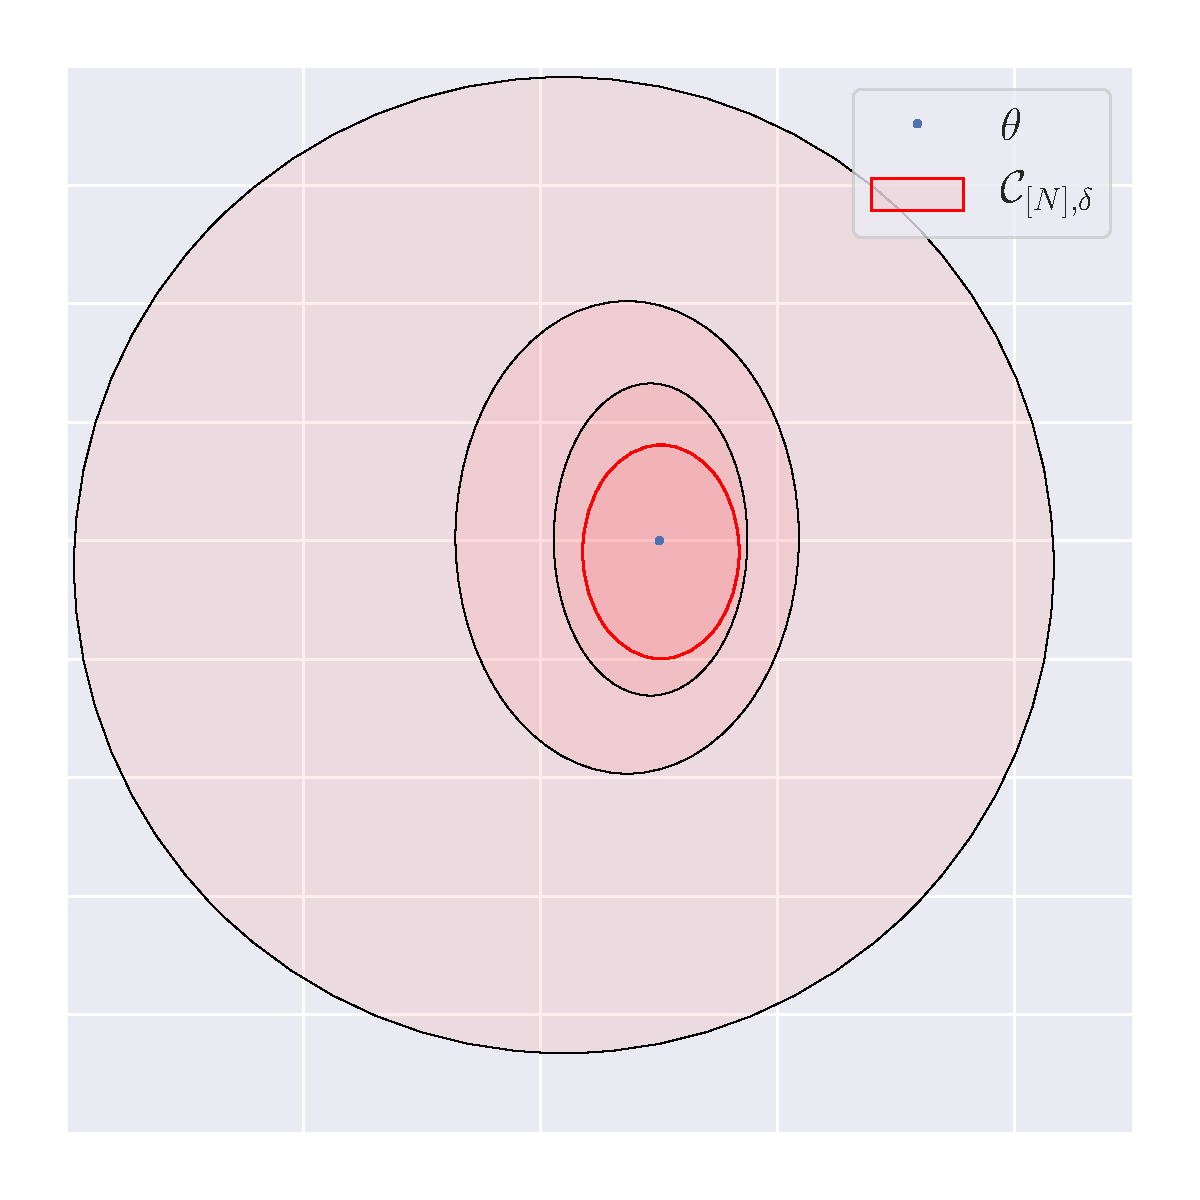
\includegraphics[trim={1cm 0 0 0}, clip, width=0.6\linewidth]{../img/ellipsoid}
	\captionof*{figure}{$C_{N,\delta}$ shrinks with the number of samples $N$.}
\end{center}

\begin{assumption}[Structure]
	\begin{equation}
	\label{eq:structure}
	A(\theta) = A + %\theta^\transp \phi \eqdef A + 
	\sum_{i=1}^d \theta_i\phi_i,
	\end{equation}
\end{assumption}

\begin{assumption}[Noise Model] Assume
	\begin{itemize}
		\item sub-Gaussian observation: $\expectedvalue \left[ \exp{\left( u^\transp \eta\right)}\right] \leq \exp{\left( \frac{1}{2} u^\transp \Sigma_p u\right)}$
		\item bounded disturbance:
		$\underline\omega(t) \leq \omega(t) \leq \overline\omega(t)$
	\end{itemize}
\end{assumption}

\bookboxx{
\begin{theorem}[Matricial version of \cite{Abbasi2011}]
	Let $\qquad \qquad \qquad \begin{aligned}[t]
	\label{eq:vector_rls}
	\theta_{N,\lambda} &= G_{N, \lambda}^{-1} \sum_{n=1}^N \Phi_n^\transp \Sigma_p^{-1} y_n,\\
	G_{N, \lambda} &= \sum_{n=1}^N \Phi_{n}^\transp\Sigma_p^{-1}\Phi_{n}  + \lambda I_d \in \Real^{d\times d}.
	\end{aligned}
	$
	
	Then, with probability at least $1-\delta$
	\begin{align}
	\label{eq:confidence-ellipsoid}
	\| \theta_{N,\lambda}  - \theta\|_{G_{N,\lambda}} \leq \beta_N(\delta), 
	\end{align}
	with 
	\[\beta_N(\delta)\eqdef \sqrt{2\ln \left(\frac{\det(G_{N,\lambda})^{1/2}}{\delta\det(\lambda I_d)^{1/2}}\right)}
	+ (\lambda d)^{1/2}S.\]
\end{theorem}
}
}

%----------------------------------------------------------------------------------------
%	Interval Prediction
%----------------------------------------------------------------------------------------
\headerbox{Interval Prediction}{name=bdp,column=1,span=2}{
	Having observed $N$ samples, given $\theta\in\cC_{N,\delta}$, we want 
	\begin{equation}
	\label{eq:inclusion-property}
	\underline{x}(t)\leq x(t)\leq\overline{x}(t), \qquad \forall t\geq t_N.
	\end{equation}
	
\begin{minipage}{0.62\textwidth}
	\bookboxx{
	\begin{proposition*}[Simple predictor of \cite{Efimov2012}]
		\begin{eqnarray}
		\dot{\underline{x}}(t) = \underline{A}^{+}\underline{x}^{+}(t)-\overline{A}^{+}\underline{x}^{-}(t)-\underline{A}^{-}\overline{x}^{+}(t) +\overline{A}^{-}\overline{x}^{-}(t) +Bu(t) + D^{+}\underline{\omega}(t)-D^{-}\overline{\omega}(t),\nonumber\\
		\dot{\overline{x}}(t) = \overline{A}^{+}\overline{x}^{+}(t)-\underline{A}^{+}\overline{x}^{-}(t)-\overline{A}^{-}\underline{x}^{+}(t)+\underline{A}^{-}\underline{x}^{-}(t)\nonumber+Bu(t) + D^{+}\overline{\omega}(t)-D^{-}\underline{\omega}(t),\nonumber
		\end{eqnarray}
		ensures the inclusion property \eqref{eq:inclusion-property}
	\end{proposition*}
    }
\end{minipage}
\hfill%
\begin{minipage}{0.38\textwidth}
	\begin{center}
		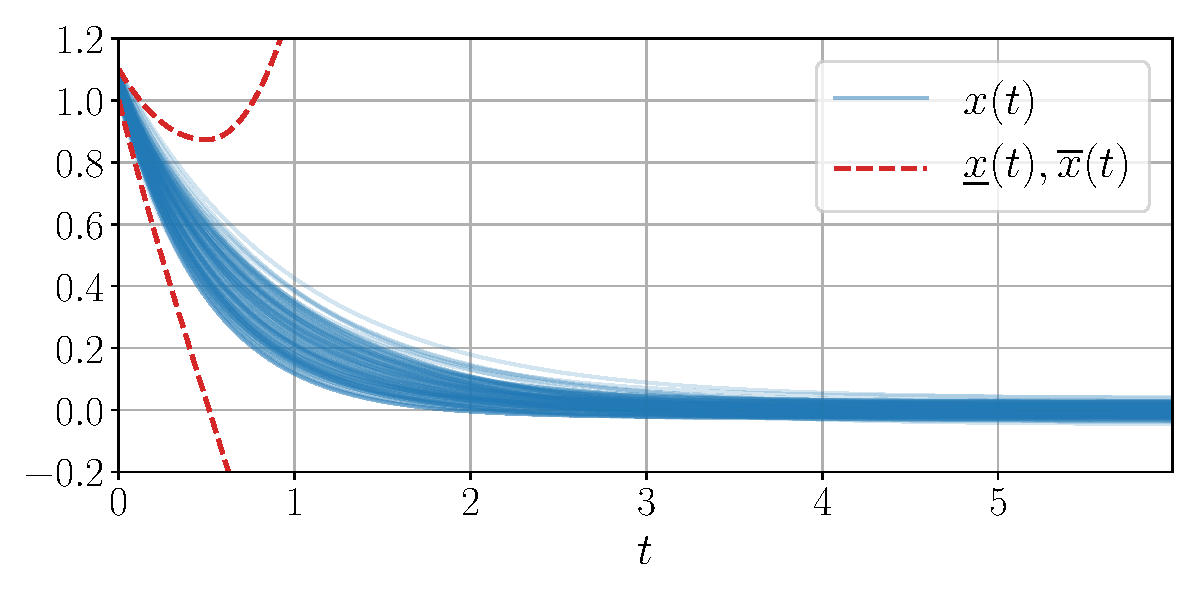
\includegraphics[trim={0 0 0 0}, clip, width=\linewidth]{./img/observer}
	\end{center}
\end{minipage}

\begin{minipage}{0.62\textwidth}
	
	\begin{assumption}
		\label{assumpt:metzler}
		There exists $Z$ orthogonal such that $Z^\transp A_N Z$ is Metzler.
	\end{assumption}
	\bookboxx{
	\begin{proposition*}[Enhanced predictor of \cite{leurent2019interval}]
		\begin{eqnarray}
		\dot{\underline{x}}(t) & = & A_{N}\underline{x}(t)-\Delta A_{+}\underline{x}^{-}(t)-\Delta A_{-}\overline{x}^{+}(t)  +Bu(t)+D^{+}\underline{\omega}(t)-D^{-}\overline{\omega}(t),\nonumber\\
		\dot{\overline{x}}(t) & = & A_{N}\overline{x}(t)+\Delta A_{+}\overline{x}^{+}(t)+\Delta A_{-}\underline{x}^{-}(t)  +Bu(t)+D^{+}\overline{\omega}(t)-D^{-}\underline{\omega}(t),\nonumber
		\end{eqnarray}
		ensures the inclusion property \eqref{eq:inclusion-property} under \Cref{assumpt:metzler}.
	\end{proposition*}
	}
\end{minipage}
\hfill%
\begin{minipage}{0.38\textwidth}
	\begin{center}
		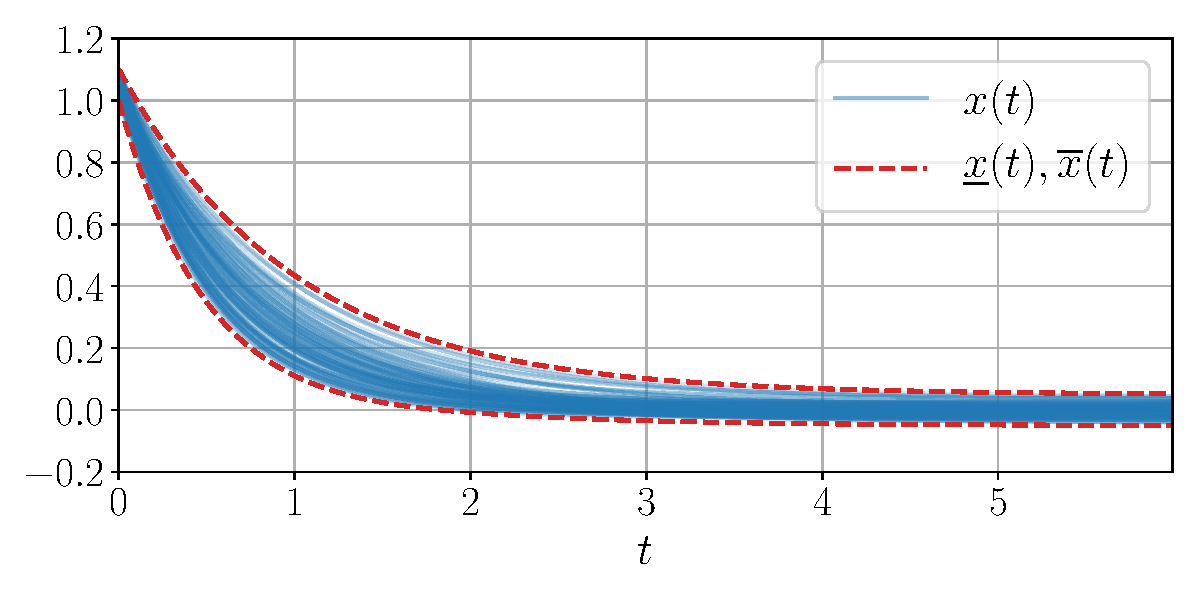
\includegraphics[trim={0 0 0 0}, clip, width=\linewidth]{./img/predictor}
	\end{center}
\end{minipage}

}
%----------------------------------------------------------------------------------------
%	Robust Control
%----------------------------------------------------------------------------------------
\headerbox{Robust Control}{name=brl,span=2,column=1,below=bdp}{ 
\begin{minipage}{0.58\textwidth}
	\begin{definition}[Surrogate objective]
		Let $\underline{x}, \overline{x}$ following \eqref{eq:inclusion-property} and
		\begin{equation*}
%		\label{eq:surrogate-objective} 
		\hat{V}^r(\bu) \eqdef \sum_{n=N+1}^\infty \gamma^n \underline{R}_n(\bu)\quad\text{where}\quad\underline{R}_n(\bu) \eqdef \min_{x\in[\underline{x}_n(\bu), \overline{x}_n(\bu)]}  R(x). %\label{eq:pessimistic-rewards}
		\end{equation*}
	\end{definition}
\end{minipage}
\hfill%
\begin{minipage}{0.4\textwidth}
\bookboxx{
	\begin{theorem}[Lower bound]
		\label{prop:lower-bound}
		\begin{equation*}
		\hat{V}^r(\bu) \leq V^r(\bu)
		\end{equation*}
	\end{theorem}
}
\end{minipage}
%\\[0.5cm]
\begin{minipage}{0.58\textwidth}
	\bookboxx{
\begin{theorem}[Suboptimality bound]
	\label{thm:minimax-regret-bound}
	Under two conditions:
	\begin{enumerate}
		\item a Lipschitz regularity assumption for the reward function $R$:
		\item a stability condition: there exist $P>0,Q_0\in\Real^{p\times p}$, $\rho>0$, and $N_0\in\Natural$ such that
		$$\forall N>N_0,\quad \begin{bmatrix}
		A_N^\transp P + P A_N^\transp + Q_0 & P|D|  \\
		|D|^\transp P & -\rho I_r \\
		\end{bmatrix}< 0;$$
	\end{enumerate}
	we can bound the suboptimality with planning budget $K$ as: with probability at least $1-\delta$,
	\begin{equation*}
	V(a_\star) - \hat{V}^r(a_K) \leq  \hler{\vph\underbrace{\Delta_\omega}_{\substack{\text{robustness to}\\ \text{disturbances}}}} + \hleb{\vph\underbrace{\cO\left(\frac{\beta_N(\delta)^2}{\lambda_{\min}(G_{N,\lambda})}\right)}_{\text{estimation error}}} + \hleg{\vph\underbrace{\cO\left(K^{-\frac{\log 1/\gamma}{\log \kappa}}\right)}_{\text{planning error}}} 
	\end{equation*}
\end{theorem}
}
\end{minipage}
\hfill%
\begin{minipage}{0.4\textwidth}
	\begin{corollary}[Asymptotic near-optimality]
		\label{cor:pe}
		Under an additional persistent excitation (PE) assumption
		\begin{align*}
%		\label{eq:pe}
		\exists \underline{\phi},\overline{\phi}>0: \forall n\geq n_0,\quad \underline{\phi}^2 \leq \lambda_{\min}(\Phi_{n}^\transp\Sigma_{p}^{-1}\Phi_{n}) \leq \overline{\phi}^2,
		\end{align*} the stability condition 2. of \Cref{thm:minimax-regret-bound} can be relaxed to its limit $A_N \to A(\theta)$ and 
		\begin{equation*}
		{\vph{\cO\left(\frac{\beta_N(\delta)^2}{\lambda_{\min}(G_{N,\lambda})}\right)}} = \cO\left(\frac{\log\left(N^{d/2}/\delta\right)}{N}\right)
		\end{equation*}

	\end{corollary}
\end{minipage}


}

%----------------------------------------------------------------------------------------
%	Multi-Model Extension
%----------------------------------------------------------------------------------------
\headerbox{Multi-Model Extension}{name=scale,span=2,column=1,below=brl}{ 


\begin{minipage}{0.7\textwidth}
	\begin{assumption}[Multi-model ambiguity]
		\label{assumpt:multi-model-ambiguity}
		$(A,\phi)$ from \eqref{eq:structure} lies within a finite set of $M$ models
	\end{assumption}

\paragraph{Model adequacy} If $y\not\in\cP^m$, the model $(A_m,\phi_m)$ can be confidently rejected.

\begin{proposition}[Robust selection]
	\label{theorem:drop-regret}
	With discrete ambiguity, the robust version of \texttt{OPD} enjoys the same regret bound as \texttt{OPD} and recovers $V^r$ exactly.
\end{proposition}


\end{minipage}
\hfill%
\begin{minipage}{0.25\textwidth}
\begin{center}
	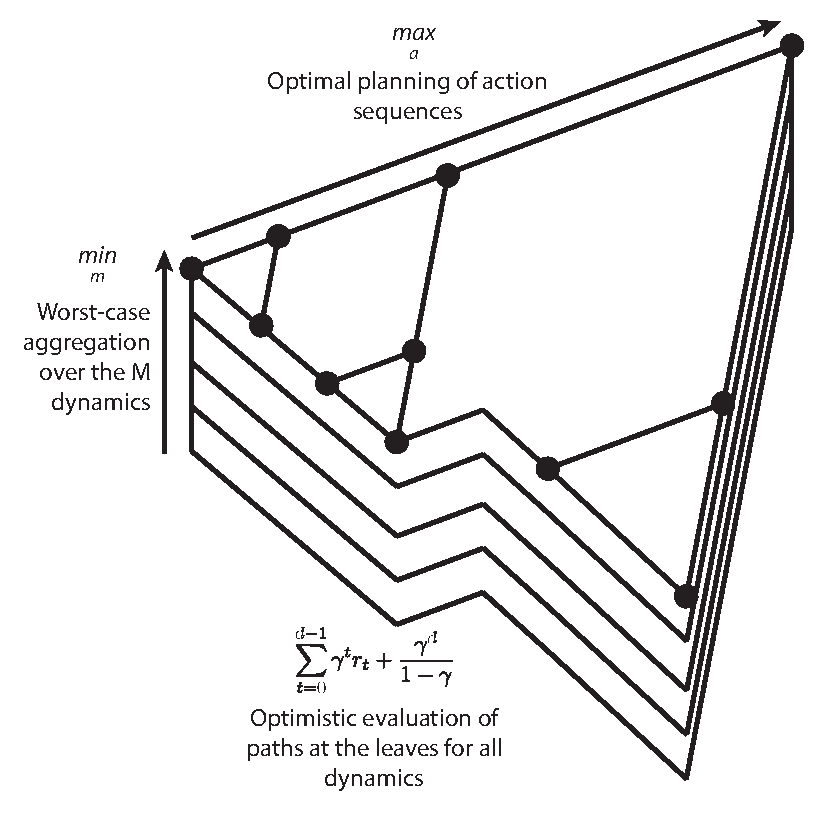
\includegraphics[width=0.8\linewidth]{../img/robust-control-tree}
\end{center}

\end{minipage}
}

%
%%----------------------------------------------------------------------------------------
%% Experiments
%%----------------------------------------------------------------------------------------
%
\headerbox{Experiments}{name=experiments,span=2,column=1,below=scale, above=bottom}{ 
	\begin{minipage}[t]{0.33\linewidth}
	\centering
	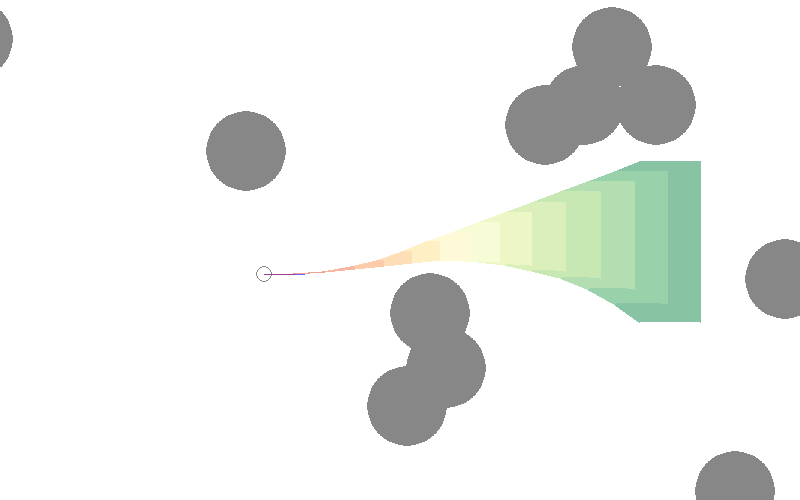
\includegraphics[trim={4cm 0 0 0}, clip, width=\linewidth]{../img/obstacle_small}
	\captionof*{figure}{Obstacle avoidance}
	\begin{tabular}{lccc}
		\toprule
		 &
		failures &
		min &
		avg $\pm$ std  \\
		\midrule
		Oracle & 0\% & {11.6} & {$14.2 \pm 1.3$} \\
		\midrule
		{Nominal} & {4\%} & {2.8} & \textbf{$\mathbf{13.8} \pm 2.0$} \\
		Robust & \textbf{0\%} & \textbf{10.4} & {$13.0 \pm 1.5$} \\
		\midrule
		DQN\footnotemark & 6\% & 1.7 & $12.3\pm2.5$ \\
		\bottomrule
	\end{tabular}
	\end{minipage}%
\hfill%
\begin{minipage}[t]{0.33\textwidth}
	\centering
	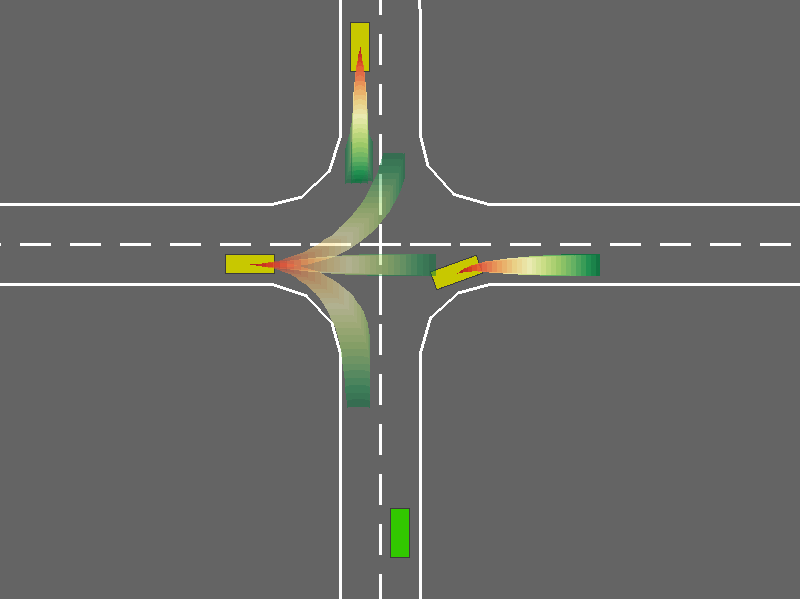
\includegraphics[width=\linewidth]{../img/highway-small}
	\captionof*{figure}{Unsignalized intersection}
	\begin{tabular}{lccc}
		\toprule
		 &
		failures &
		min &
		avg $\pm$ std  \\
		\midrule
		Oracle & 0\% & {6.9} & $7.4 \pm 0.5$ \\
		\midrule
		{Nominal 1} & 4\% & {5.2} & $\mathbf{7.3} \pm 1.5$ \\
		{Nominal 2} & 33\% & {3.5} & $6.4 \pm 0.3$ \\
		Robust & \textbf{0\%} & \textbf{6.8} & $7.1 \pm 0.3$ \\
		\midrule
		DQN\footnotemark[\value{footnote}] & 3\% & 5.4 & $6.3\pm0.6$ \\
		\bottomrule
	\end{tabular}
\end{minipage}
	\begin{minipage}[t]{0.31\textwidth}
	\centering
	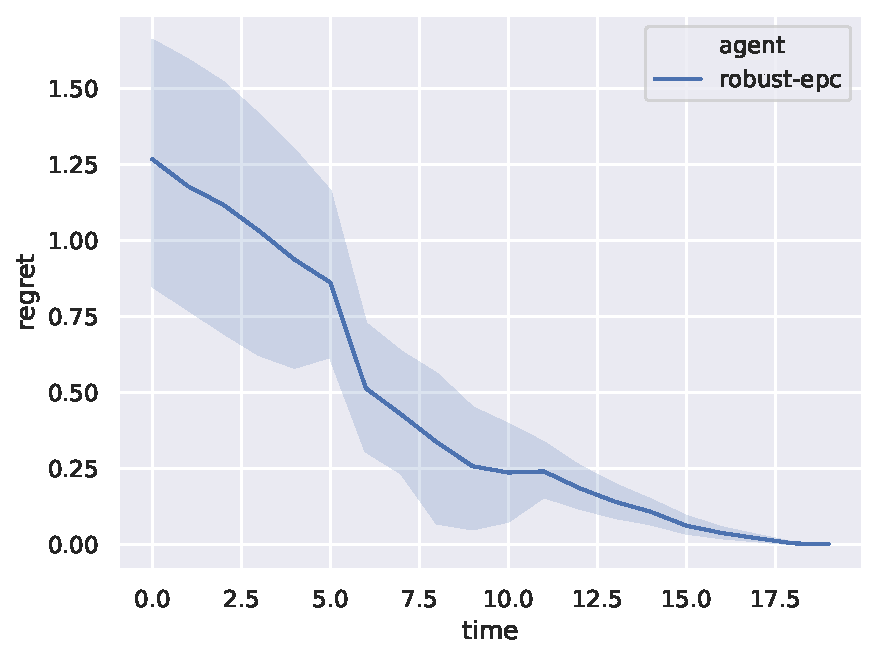
\includegraphics[trim={0 0.2cm 0 0.2cm}, clip, width=\linewidth]{../img/regret.pdf}
\captionof*{figure}{Mean regret with respect to $N$}	
	\end{minipage}%
\footnotetext[1]{After training on 3000 episodes} 
	
}



%----------------------------------------------------------------------------------------
%	Acknowledgements
%----------------------------------------------------------------------------------------
%\headerbox{Acknowledgements}{name=ack,column=0,span=1,below=bopt}{
%This work has been supported by CPER Nord-Pas de Calais/FEDER DATA Advanced data science and technologies 2015-2020, the French Ministry of Higher Education and Research, INRIA, and the French Agence Nationale de la Recherche (ANR).
%}


%----------------------------------------------------------------------------------------
%	References
%----------------------------------------------------------------------------------------
\headerbox{References}{name=refs,column=0,span=1,below=bopt, above=bottom}{
    {
    \AtNextBibliography{\footnotesize}
    \setlength{\bibitemsep}{3pt}
    \printbibliography[heading=none]
    }
}


\end{poster}

\end{document}


